%
\documentclass{sigchi}

% Use this section to set the ACM copyright statement (e.g. for
% preprints).  Consult the conference website for the camera-ready
% copyright statement.

% Copyright
\CopyrightYear{2016}
%\setcopyright{acmcopyright}
\setcopyright{acmlicensed}
%\setcopyright{rightsretained}
%\setcopyright{usgov}
%\setcopyright{usgovmixed}
%\setcopyright{cagov}
%\setcopyright{cagovmixed}
% DOI
\doi{http://dx.doi.org/10.475/123_4}
% ISBN
\isbn{123-4567-24-567/08/06}
%Conference
\conferenceinfo{CHI'16,}{May 07--12, 2016, San Jose, CA, USA}
%Price
\acmPrice{\$15.00}

% Use this command to override the default ACM copyright statement
% (e.g. for preprints).  Consult the conference website for the
% camera-ready copyright statement.

%% HOW TO OVERRIDE THE DEFAULT COPYRIGHT STRIP --
%% Please note you need to make sure the copy for your specific
%% license is used here!
% \toappear{
% Permission to make digital or hard copies of all or part of this work
% for personal or classroom use is granted without fee provided that
% copies are not made or distributed for profit or commercial advantage
% and that copies bear this notice and the full citation on the first
% page. Copyrights for components of this work owned by others than ACM
% must be honored. Abstracting with credit is permitted. To copy
% otherwise, or republish, to post on servers or to redistribute to
% lists, requires prior specific permission and/or a fee. Request
% permissions from \href{mailto:Permissions@acm.org}{Permissions@acm.org}. \\
% \emph{CHI '16},  May 07--12, 2016, San Jose, CA, USA \\
% ACM xxx-x-xxxx-xxxx-x/xx/xx\ldots \$15.00 \\
% DOI: \url{http://dx.doi.org/xx.xxxx/xxxxxxx.xxxxxxx}
% }

% Arabic page numbers for submission.  Remove this line to eliminate
% page numbers for the camera ready copy
% \pagenumbering{arabic}

% Load basic packages
\usepackage{balance}       % to better equalize the last page
\usepackage{graphicx}      % for EPS, load graphicx instead 
\usepackage[T1]{fontenc}   % for umlauts and other diaeresis
\usepackage{txfonts}
\usepackage{mathptmx}
\usepackage[pdflang={en-US},pdftex]{hyperref}
\usepackage{color}
\usepackage{booktabs}
\usepackage{textcomp}
\usepackage{pgfplots}
\usepackage{caption, subcaption, graphics}



% Some optional stuff you might like/need.
\usepackage{microtype}        % Improved Tracking and Kerning
% \usepackage[all]{hypcap}    % Fixes bug in hyperref caption linking
\usepackage{ccicons}          % Cite your images correctly!
% \usepackage[utf8]{inputenc} % for a UTF8 editor only

% If you want to use todo notes, marginpars etc. during creation of
% your draft document, you have to enable the "chi_draft" option for
% the document class. To do this, change the very first line to:
% "\documentclass[chi_draft]{sigchi}". You can then place todo notes
% by using the "\todo{...}"  command. Make sure to disable the draft
% option again before submitting your final document.
\usepackage{todonotes}

% Paper metadata (use plain text, for PDF inclusion and later
% re-using, if desired).  Use \emtpyauthor when submitting for review
% so you remain anonymous.
\def\plaintitle{Aparecium: Inking Interactions for Slide Presentations}
\def\plainauthor{First Author, Second Author, Third Author,
  Fourth Author, Fifth Author, Sixth Author}
\def\emptyauthor{}
\def\plainkeywords{Authors' choice; of terms; separated; by
  semicolons; include commas, within terms only; required.}
\def\plaingeneralterms{Documentation, Standardization}

% llt: Define a global style for URLs, rather that the default one
\makeatletter
\def\url@leostyle{%
  \@ifundefined{selectfont}{
    \def\UrlFont{\sf}
  }{
    \def\UrlFont{\small\bf\ttfamily}
  }}
\makeatother
\urlstyle{leo}

% To make various LaTeX processors do the right thing with page size.
\def\pprw{8.5in}
\def\pprh{11in}
\special{papersize=\pprw,\pprh}
\setlength{\paperwidth}{\pprw}
\setlength{\paperheight}{\pprh}
\setlength{\pdfpagewidth}{\pprw}
\setlength{\pdfpageheight}{\pprh}

% Make sure hyperref comes last of your loaded packages, to give it a
% fighting chance of not being over-written, since its job is to
% redefine many LaTeX commands.
\definecolor{linkColor}{RGB}{6,125,233}
\hypersetup{%
  pdftitle={\plaintitle},
% Use \plainauthor for final version.
%  pdfauthor={\plainauthor},
  pdfauthor={\emptyauthor},
  pdfkeywords={\plainkeywords},
  pdfdisplaydoctitle=true, % For Accessibility
  bookmarksnumbered,
  pdfstartview={FitH},
  colorlinks,
  citecolor=black,
  filecolor=black,
  linkcolor=black,
  urlcolor=linkColor,
  breaklinks=true,
  hypertexnames=false
}

% create a shortcut to typeset table headings
% \newcommand\tabhead[1]{\small\textbf{#1}}
\newcommand{\interface}[0]{\textit{Aparecium}}

\newcommand {\wil}[1]{{\color{green}\bf{WL: #1}\normalfont}}
\newcommand {\val}[1]{{\color{blue}\bf{VS: #1}\normalfont}}
\newcommand {\fd}[1]{{\color{magenta}\bf{FD: #1}\normalfont}}

% End of preamble. Here it comes the document.
\begin{document}

\title{\plaintitle}

%\numberofauthors{3}
%\author{%
%  \alignauthor{Leave Authors Anonymous\\
%    \affaddr{for Submission}\\
%    \affaddr{City, Country}\\
%    \email{e-mail address}}\\
%  \alignauthor{Leave Authors Anonymous\\
%    \affaddr{for Submission}\\
%    \affaddr{City, Country}\\
%    \email{e-mail address}}\\
%  \alignauthor{Leave Authors Anonymous\\
%    \affaddr{for Submission}\\
%    \affaddr{City, Country}\\
%    \email{e-mail address}}\\
%}

\maketitle

\begin{abstract}
    We present \interface, a presentation interface that helps presenters deliver flexible and engaging presentations by combining the advantages of electronic slides with inking. In \interface, presenters use inking interactions to deliver slide presentations. With inking, presenters can (1) reveal pre-authored content to the audience, (2) make annotations on top of the slide, and (3) adjust to slide layout to create blank space. Inking enables presenters to have flexibility and fine-grained control over the content and pace of the presentation, while pre-authored slides help improve its aesthetics and organization. The findings from our user study suggest that \interface\ improves presentation quality without increasing the burden on the presenter at authoring or presentation time. Especially for text-centered or process-driven content, both audiences and presenters preferred presentations delivered using \interface.
\end{abstract}

\category{H.5.m.}{Information Interfaces and Presentation
  (e.g. HCI)}{Miscellaneous} \category{See
  \url{http://acm.org/about/class/1998/} for the full list of ACM
  classifiers. This section is required.}{}{}

\keywords{\plainkeywords}
\section{Introduction}

Presentation technology has a significant impact on how we learn and teach. Today, there are largely two modes of presentation technology used in classrooms: inking on surface and projecting prepared slides. \\
35mm slide projectors first came into widespread use during the 1950s, but recently the popularization of slide authoring tools like PowerPoint, Keynote or Google Slides made electronic slides became much more common and easy. Despite its advantages--e.g., easy to share, archive, include multimedia--slides also have critical drawbacks. 
(1) Slide presentations are \textbf{rigid}: All of the editing and preparation is done ahead of time and fixed at the time of the presentation. There is no flexibility to change the order or content of the presentation during performance. 
(2) Slide presentations are \textbf{discrete}: Information is divided and presented in chunks. First the entire content is divided into separate slides, and within each slide text or graphics are presented in chunks, usually using animation effects. The appearance or transition of information is sudden and discrete.
(3) Slide presentations are \textbf{indirect}: The action of the presenter (i.e., pressing "next" to advance the slide) is removed from the effect on the content. For example, this makes it easy for presenters to forget or skip an animation sequence.\\

Inking on surface is an alternative or supplement. Inking includes blackboard or transparency and overhead projector. Inking complements the characteristics of slides. Inking is flexible, continuous and direct, but this has its own downsides.
(1) Inking is \textbf{flexible} since all of the presentation is done on the fly. But, this means there is a lot of cognitive overload for the presenter in order to decide the content, layout and order of the presentation on the fly. 
(2) Inking is \textbf{continuous}: Since the presenter writes or draws in real time, content is presented in a continuous way. This is useful for information-loaded contents or where order within the content is important, for example, derivation of a math formula or describing a temporal process. However, it is difficult to time the presentation or present a lot of information. Inking lectures tend to be slower paced [citation].
Finally, (3) inking is direct. Users actions (drawing, erasing, underlying) are all directly translated into content. This requires a lot of attention, skill on the part of the presenter. Often, presenters are reluctant to write because of their messy handwriting. Also content is limited to text or simple diagrams.

There are previous work to blend the two modes. [Classroom Presenter] or recent versions of [PowerPoint] allow you to ink on slides. But these tools treat the two modes as separate. Ink and slide remain separate layers retaining their characteristics. The slide layer remains rigid and fixed; and ink is placed on top of it.

\textbf{We propose inking as a main modality to present slide contents in a continuous, flexible and direct manner}. By inking over to reveal content, users regain flexibility, continuity and direct control over the presentation style, without losing the elegance of the prepared content.  


\section{Related Work}

\textbf{Presentation Software.} The vast majority of presentations today are created with WYSIWYG slide authoring software like PowerPoint \cite{powerpoint2017}, Keynote \cite{keynote2017} and Google Slides \cite{googleslides2017}. 
%
While these tools provide a broad range of content creation features, including the ability to add animation effects to slide elements, 
they offer limited flexibility or control at presentation time. 
%
Presenters can only advance linearly through the predefined sequence of animations and slide transitions.

\textbf{Nonlinear Presentations.} To address this shortcoming, previous research investigates how to support nonlinear paths though a presentation. Moscovich et al \cite{moscovich2004customizable} organize slides into nested directed graphs and allow presenters to choose between multiple paths on the fly. Similarly, Drucker et al. \cite{drucker2006comparing} suggest a method to compare and manage multiple slide presentation paths. Fly \cite{lichtschlag2009fly} and CounterPoint \cite{good2002zoomable} allow spatial navigation by embedding slides on an infinite canvas and employing zooming user interfaces (ZUIs). Prezi \cite{prezi2017} is a commercial, online platform for authoring zoomable presentations. Whereas this work focuses on navigating between slides or the presentation as a whole, the interactions in our work provide flexibility and control within each slide.

\textbf{Controlling Presentations.} Other work explores alternative techniques to control slide presentations. Palette \cite{nelson1999palette} uses physical cards to provide random access to slides, Baudel and Beaudouin-Lafon \cite{baudel1993charade} propose hand gestures, and Cheng and Pulo \cite{cheng2003direct} use an infrared laser pointer to control presentations. Cao et al. \cite{cao2005evaluation} perform a systematic user study comparing different interaction techniques, including hand gestures, laser pointer and standard mouse/keyboard input. Our work suggests inking interactions as the main mode to present slides.

\textbf{Inking on Digital Documents.} Many systems \cite{yoon2014richreview, marshall1999collaborating, hardock1993marking} support digital inking to make annotations on top of documents. Perhaps most similar in spirit to our work are systems that integrate digital ink with prepared slides. Anderson et al.~\cite{anderson2007classroom} propose Classroom Presenter, a distributed presentation system that allows instructors and students to share digital ink on top of electronic slides. Recently, PowerPoint and Keynote added support for presenters to ink in presentation mode as well. SMART is another commercial system that supports inking and projected material using an interactive whiteboard \cite{smarttech2017}. While all of these systems combine slides with inking, the underlying slide content remains inherently separate from the ink on top. In contrast, in our system, presenters use ink to reveal underlying slide elements in a flexible, fine-grained way at presentation time.
%\val{This sentence would also benefit from clarification of inking: as a gesture vs. output.} 
%\wil{Is that better?}

\textbf{Beautifying Ink.} To further assist freeform digital inking, researchers have experimented with different methods to beautify the user's ink strokes. Beautification is applied to meet the requirements of specific scenarios, such as geometric diagrams \cite{igarashi1998pegasus, hse2005recognition, fivser2015shipshape}, hand-drawn pictures~\cite{xie2014portraitsketch, limpaecher2013}, handwriting \cite{zitnick2013handwriting} or mathematical diagrams~\cite{laviola2007mathpad}. Our work does not modify the user's ink stroke per se, but we achieve a similar effect by making the ink stroke disappear gradually and revealing the underlying pre-authored slide content instead.

\section{Current Practice and Needs}
To learn about current practice and unsupported needs in presentation technology, we conducted multiple rounds of interviews with classroom lecturers, online lecturers, graduate student TAs, and undergraduate students, with varied experiences in giving and listening to presentations. 
%
We also consulted existing literature comparing different types of presentation software.
%
From this analysis, we summarize the key findings that informed the design of our system.

\textbf{Flexibility in presentations is preferred for interactive or informal settings.} For settings such as research conferences or business meetings with tight time constraints and little room for audience interaction, people prefer to give highly scripted presentations with electronic slides. However, for settings such as lectures, tutoring sessions, or brainstorming meetings, presenters like to have some flexibility and often use inking as part of their presentations. Common strategies include using a blackboard or projecting slides/transparencies onto a board and inking on top of them. Several lecturers purposefully leave blank spaces on their slides to fill in by inking during the lecture. %Inking allows presenters to draw attention to content by writing or annotating in real time, to modify the order in which content is presented, or in some cases, to modify the content itself based on audience input or feedback.

\textbf{Presenters want flexibility over prepared contents rather than complete improvisation.} Even for informal settings, presenters have the bulk of the content planned and prepared beforehand, in the form of lecture notes, worksheets or slides. Thus, the type of flexibility that presenters want is the ability to make small-scale adjustments on-the-fly, such as omitting part of the content, adding minor changes such as a line of text or annotations, or changing the order of the contents. Inking is often used to this effect. 
%\wil{This is repetitive with the last sentence in the previous paragraph.}

\textbf{Pacing is important and context dependent.} 
The choice of tool also affects the pace of the presentation. Electronic slides are useful for displaying information quickly, which may explain why presenters prefer them for time-constrained settings. Inking takes time, but it allows presenters to have fine-grained control over the pace of the presentation. Depending on the subject matter, the pace of real time writing also makes it easier to follow for the audience. For example, when describing sequential processes like solving a math problem or explaining a complex diagram, both presenters and viewers find it more effective to write them out step-by-step in real-time. Slide animations can simulate this effect, but setting up fine-grained animations is tedious. As a result, animated presentations typically include a very coarse set of discrete steps. 

\textbf{Visual aesthetics matter but are difficult to achieve with inking.} Both as a presenter and as an audience, people frequently mentioned better visual aesthetics as an advantage of slides over inking. Presenters are often not satisfied with or even embarrassed by their own handwriting. They pointed out that it is even more difficult to write while talking at the same time. Even small operations, such as changing the pen color, seem burdensome during the lecture, as noted by Anderson\cite{anderson2004study}. 
% \wil{Previous two sentences don't seem to be about aesthetics. Is there a separate observation to make about timing? Or could this go into the first observation on context-dependent flexibility?}
%
From a viewing perspective, people like the legibility and organization that pre-authored slides provide. As \cite{frey2002learners} also mention, sometimes audiences even felt that lecturers are better prepared when they present using electronic slides. 
%\wil{For the two points with citations, are these things that also came up in your interviews, or are you just citing previous findings? If the former, we should try to make that clear, as I did with the Anderson reference above.}
\begin{figure*}[t!]
    \centering
    \begin{subfigure}[t]{0.32\textwidth}
        \centering
        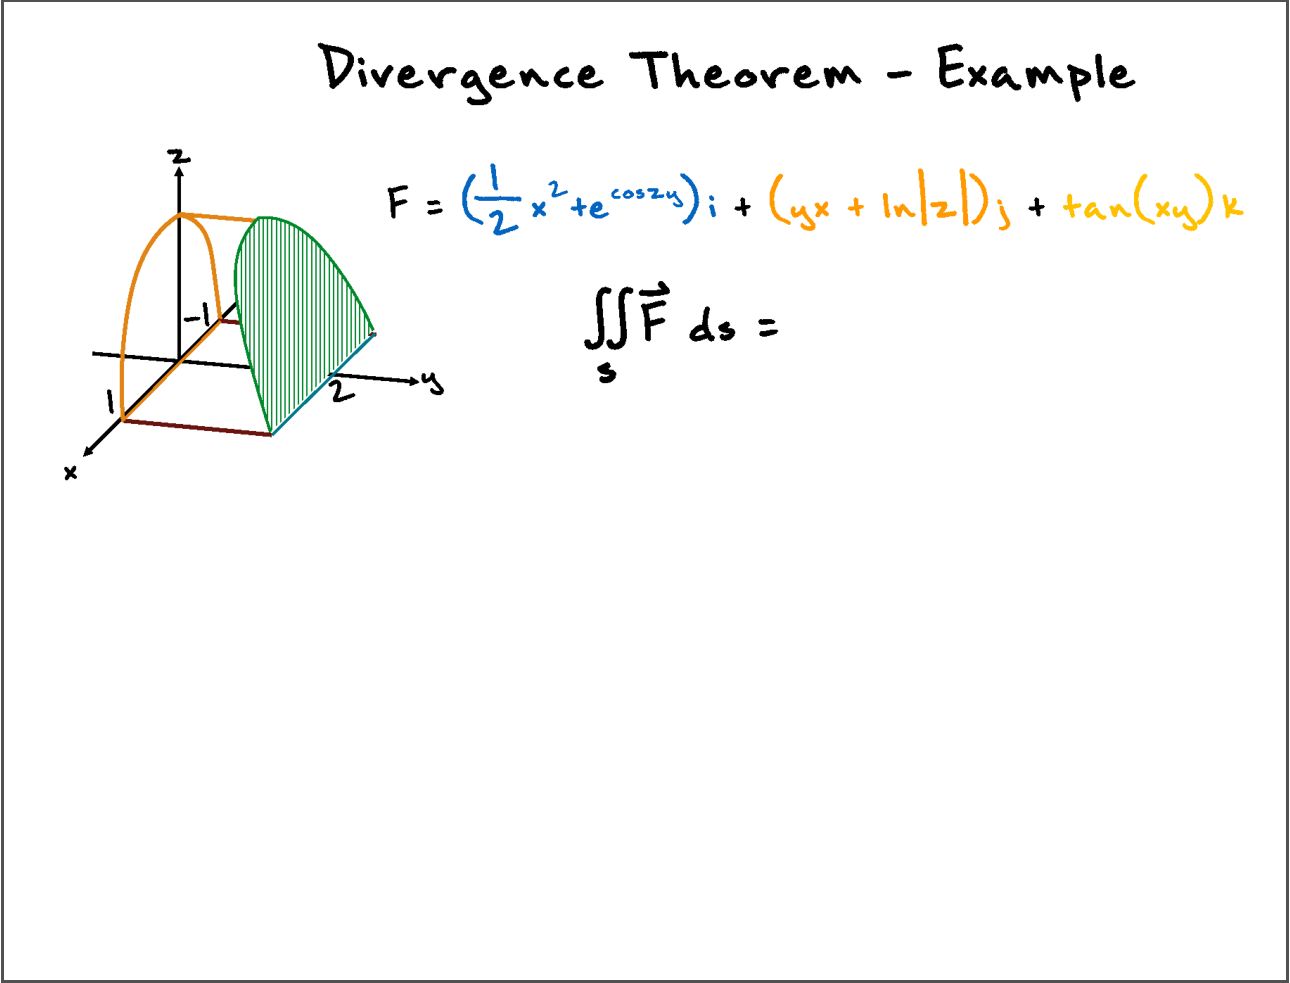
\includegraphics[width=1\columnwidth]{figures/videoslide1}
        \caption{Background (Audience View)}
    \end{subfigure}%
    ~ 
    \begin{subfigure}[t]{0.32\textwidth}
        \centering
        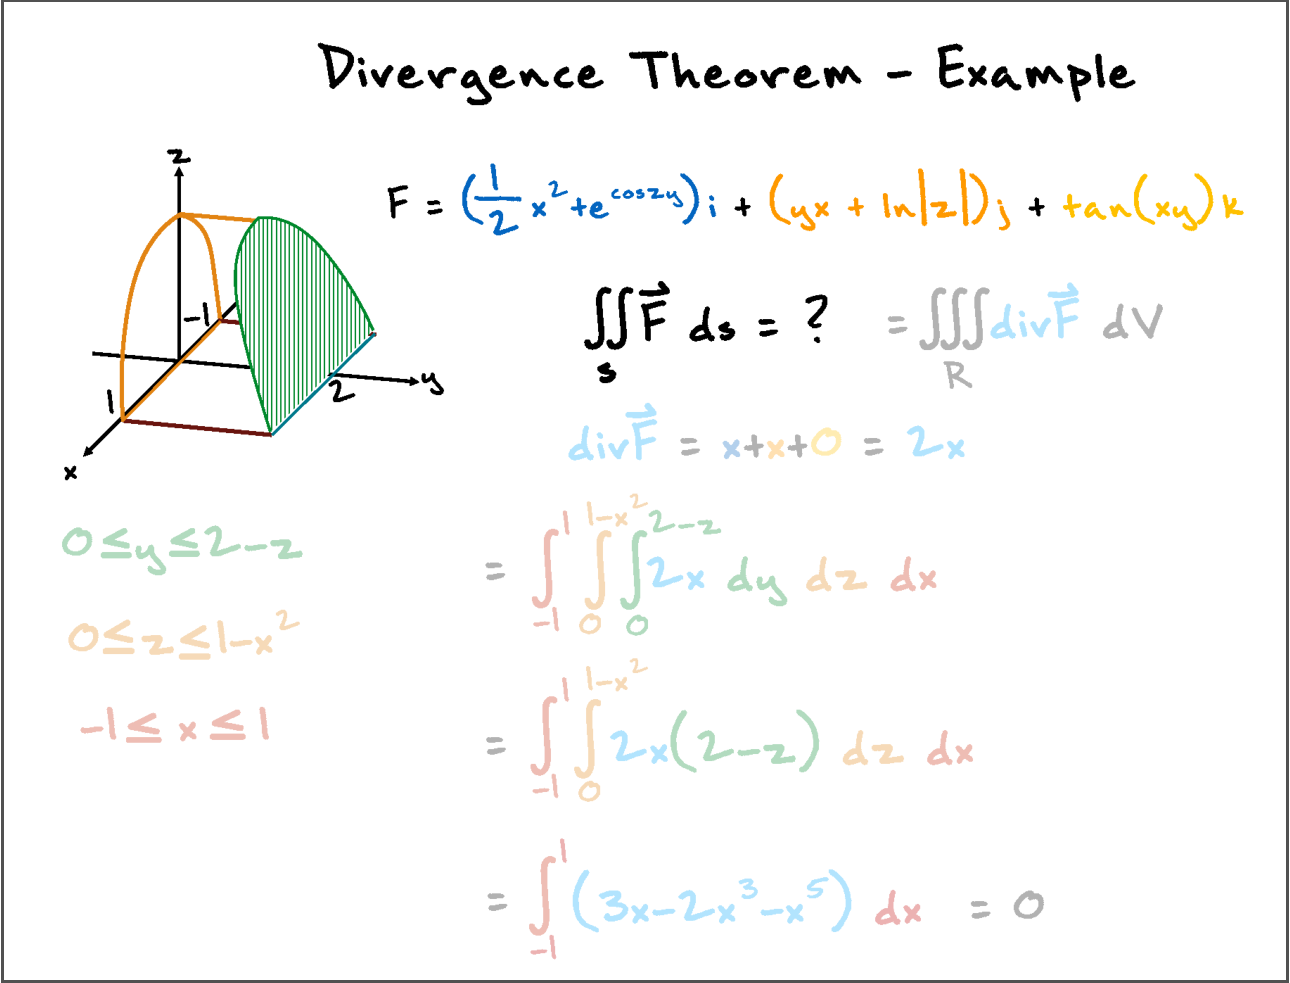
\includegraphics[width=1\columnwidth]{figures/videoslide2}
        \caption{Background + Foreground (Presenter View)}
    \end{subfigure}
    ~
        \begin{subfigure}[t]{0.32\textwidth}
        \centering
        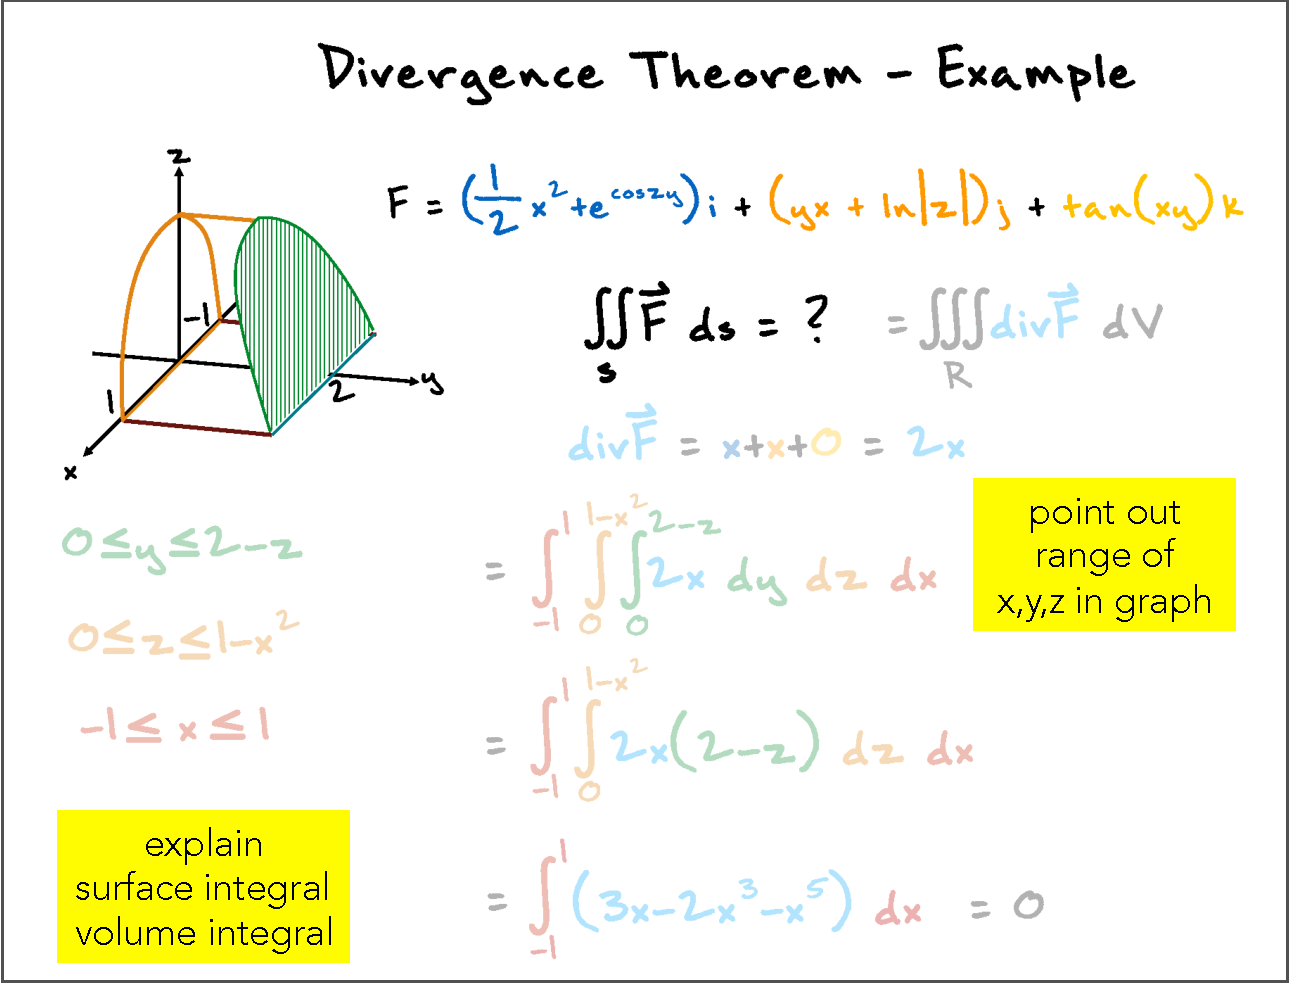
\includegraphics[width=1\columnwidth]{figures/videoslide3}
        \caption{Background + Foreground + Notes}
    \end{subfigure}
    \caption{Slide Layers in \interface. Slides are separated into foreground and background layers. \textbf{(a)} The background layer is always visible and it is what the audience sees initially. \textbf{(b)} The foreground layer is initially only visible on the presenter view, and is faded to distinguish it from the background. Presenters can reveal parts of it to the audience during delivery. The revealed parts appear on the audience view and becomes unfaded on the presenter view. \textbf{(c)} Optionally, presenters can also have the notes layer, which is only visible on the presenter view and acts as transparent speaker notes placed on top of the slides. }
    \label{fig:slidelayers}
\end{figure*}
\section{Design Goals}

The above findings highlight the complementary attributes of electronic slides and inking. While slides are typically more organized and aesthetically pleasing, inking offers greater flexibility and fine-grained control at presentation time.
%
Our aim is to develop a presentation interface that combines the advantages of both existing technologies without increasing the burden on the presenter at authoring and presentation time.
%
More specifically, our system should achieve the following design goals. The first two goals are concerned with improving the presentation quality, while the last goal involves reducing the presenters' effort. 

\textbf{Maximize organization and aesthetics through pre-authored contents.} In order to improve presentation quality, we want to take full advantage of contents that presenters prepare beforehand. Pre-authored contents can help achieve visual aesthetics. It also \textit{forces} the presenter to organize the presentation ahead of time. 
 
\textbf{Maximize flexibility and fine-grained control during presentation delivery.} Presenters should have fine control over what visual content to present, and also when, how much, and how fast to present them. Moreover, these decisions need not be made ahead of time; instead, presenters should be able to implement and adjust them while delivering, according to the content and audience. 

\textbf{Minimize presenter effort during delivery as well as during preparation.} We want to give presenters more control, but without increasing their burden. Interactions during delivery should be as simple and natural as possible. Similarly, preparation itself should not take more effort than, for example, authoring regular slides. Moreover, presenters should be allowed to focus more on preparing the content itself rather than, for instance, spending time to setup animations effects for delivery. 

%These design goals are expressed in \interface in the following ways. 



\section{Design of \interface}
\wil{Before getting into the details of the method, I think we should
  describe the key aspects of our design (fine-grained reveal and
  space manipulation, right?) and connect them to our design principles.}

\interface uses pre-authored slides, prepared by the presenters ahead of time, in pretty much the same way as they would for a regular electronic presentation. The slides help presenters organize their material and to improve visual aesthetics. However, unlike traditional electronic slides, presenters do not specify beforehand when, how, or in which order the elements in the slide will appear (i.e., animation effects). Instead, they simply specify which elements will be displayed to the audience immediately versus which elements will be revealed in real time. 

\interface's main mode of interaction during delivery is inking. Inking has three functions depending on the context: it can (1) reveal pre-authored slide elements to the audience, (2) add ink strokes on top of the slide, or (3) adjust the slide layout by creating blank space. Inking allows presenters to have flexibility and fine-grained control over when, how much, and how fast to reveal elements on the slide. Presenters can also add extra writings or annotations on top of pre-authored elements, and create blank space if necessary. All of these interactions are implemented as modeless pen interactions. 
 
\subsection{Slide authoring}
\val{Figure showing example of background / foreground / notes}
Slides in \interface can be authored using any existing slide presentation software (e.g., PowerPoint, Keynote, GoogleSlides). They can include typed text or images, as well as, hand drawn ink strokes. Instead of specifying animation effects on these slide elements, presenters separate them into two layers for each slide. The background layer is always visible and it is what the audience sees initially. The foreground layer is initially only visible on the presenter view, but presenters can reveal parts of it to the audience during delivery. ]\val{Presenters also have the option of preparing a third layer, the notes layer, which is only visible on the presenter view and serves as a transparent lecture note placed on top of the slides.} Layers in \interface are represented as bitmap images. 

\subsection{Inking during delivery}
During delivery, presenters ink on top of the pre-authored slides. Inking has three different functions depending on the context. 
\textbf{Reveal}
If the presenter inks over \val{around? I want to somehow convey that inking over does not have to be precise: i.e. on top of the pixels} foreground pixels that have not been revealed to the audience yet, these and neighboring foreground pixels are revealed to the audience in the following way. For each point, $s_i$ in the user's ink stroke, the closest foreground pixel, $p_i$ is computed. If $p_i$ is close enough to $s_i$, a flood-fill is performed starting from $p_i$ to neighboring foreground pixels. The extent of the flood-fill is limited by thresholds on (1) the distance from $p_i$, and (2) the color difference from $p_i$. In order to give presenters finer-grained control over the extent of the reveal, the thresholds vary according to the velocity of the presenter's ink stroke. If the presenter inks slowly, only a small neighborhood close to the original stroke is revealed. This is useful when the presenter wants to simulate writing in real-time, and reveal, for example, a part of a character or a diagram. If the presenter inks quickly (e.g., scribbles), a larger neighborhood is revealed. This allows presenters, for instance, to swiftly reveal an entire image or a line of text without having to ink over them precisely.  \val{Figure showing user tracing over a formula, one character at a time}

\textbf{Annotate}
If the presenter inks over empty pixels on the foreground, or if the foreground pixels around the stroke has already been revealed previously, the ink stroke appears on top of the foreground layer as is. \interface computes the average color of the slide around the stroke and sets the ink color to a complementary color so that the ink stands out from the slide. \val{Figure of annotation over revealed element and annotation on empty background}. 

\textbf{Create Space}
Sometimes, presenters may want extra space to insert new content in the slide, for example, to add an item to an existing list, a word in a sentence, or an extra line of explanation. These situations can arise as a result of a mistake in the preparation phase (e.g., the presenter forgets to list an item), as well as from presenter-audience interaction (e.g., the audience requests extra explanation). \interface allows presenters to create empty space from ink strokes. First, the presenter draws a curve where the empty space is to be created. At the end of the curve, if the presenter holds down the pen for more than 0.5 seconds, the curve turns into a red dashed stroke, indicating that the presenter can start expanding the space around the curve. As the presenter moves the pen along one of the axis-aligned directions, empty space is created and expanded from the curve in that direction.  As the space grows, the foreground content is shifted accordingly. \val{Figure showing the steps.}

\section{User Evaluation}
\begin{figure}[t!]
    \centering
    \begin{subfigure}[t]{1\columnwidth}
        \centering
        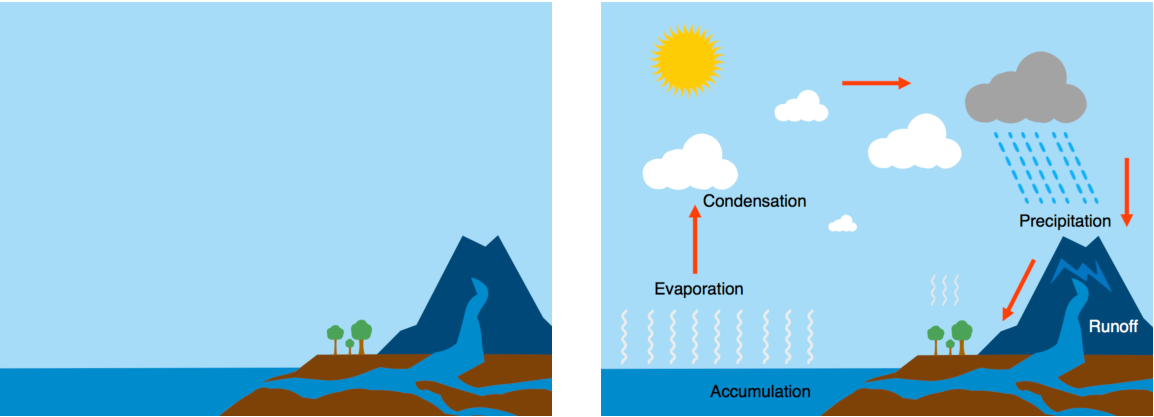
\includegraphics[width=1\columnwidth]{figures/watercycle}
        \caption{Lorem ipsum}
    \end{subfigure}
    ~ 
    \begin{subfigure}[t]{0.48\columnwidth}
        \centering
        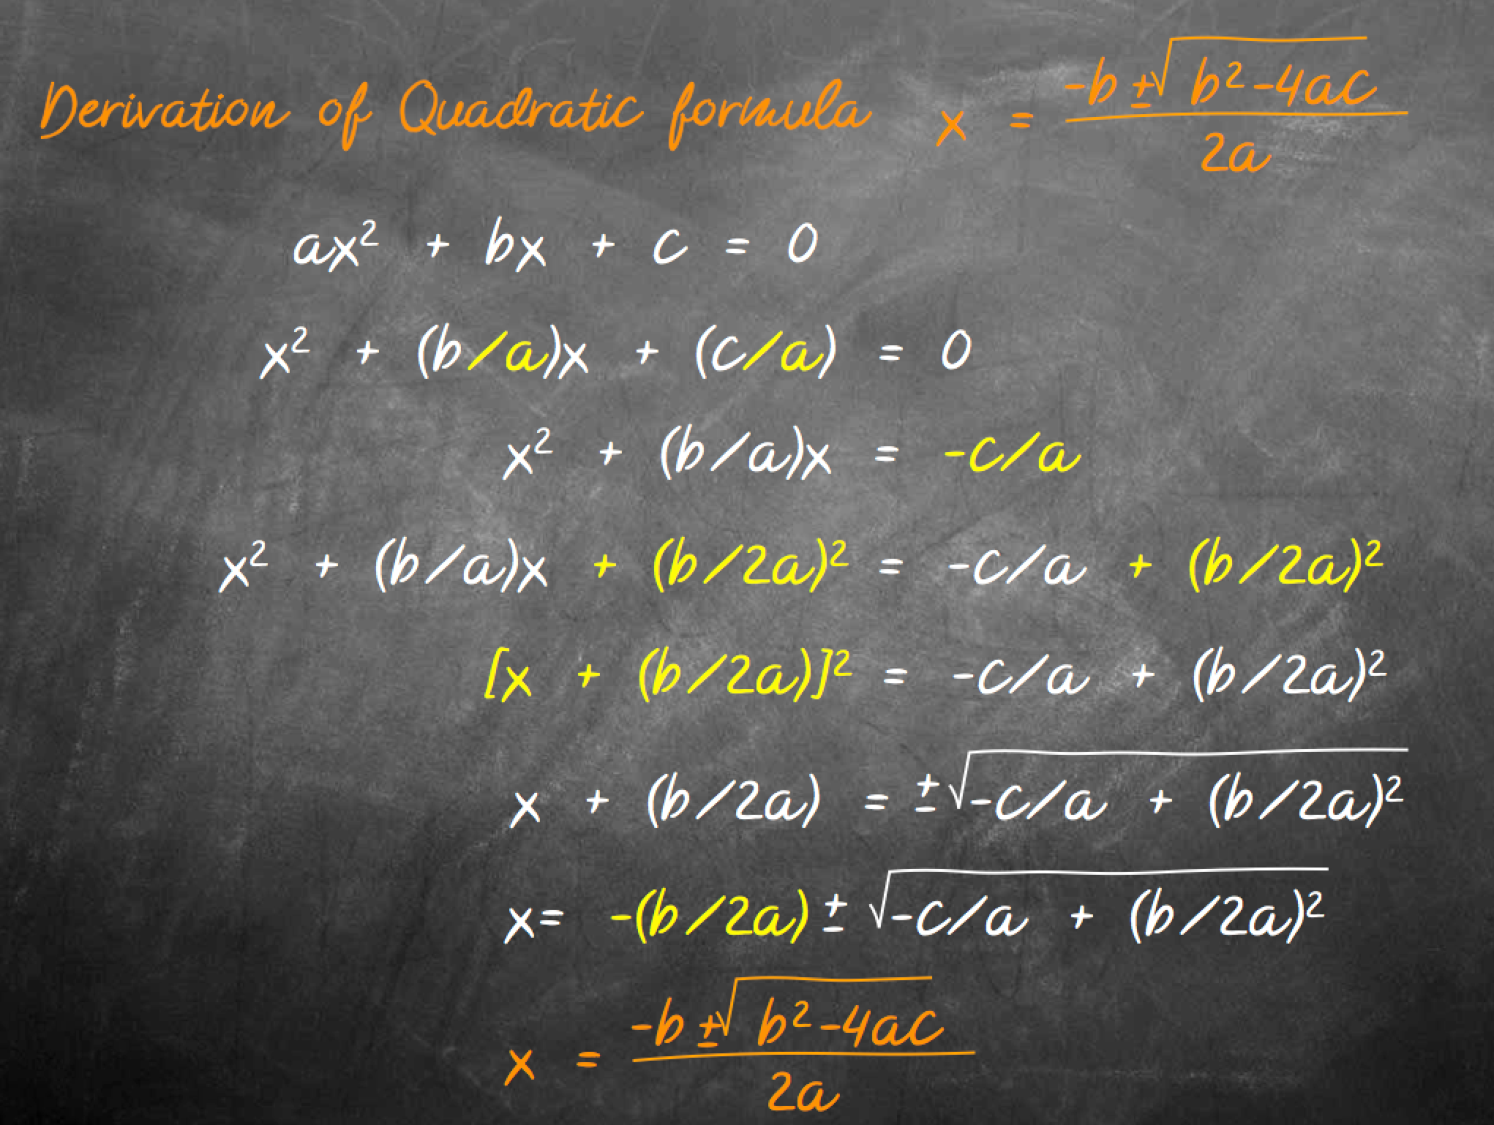
\includegraphics[width=1\columnwidth]{figures/quadformula}
        \caption{Lorem ipsum}
    \end{subfigure}  
    ~
    \begin{subfigure}[t]{0.48\columnwidth}
        \centering
        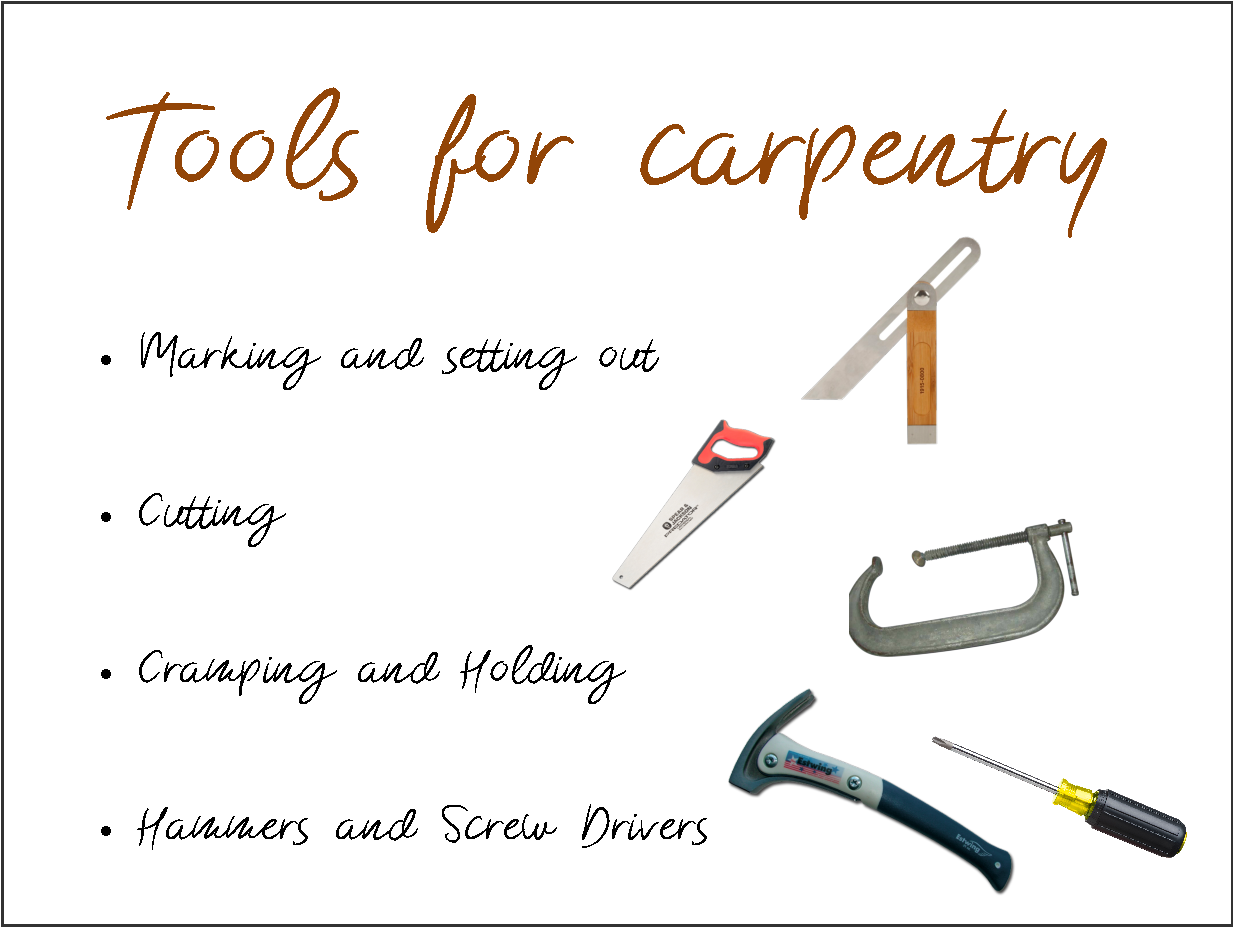
\includegraphics[width=1\columnwidth]{figures/tools}
        \caption{Lorem ipsum}
    \end{subfigure}  
    \caption{Evaluation slides}
\end{figure}

We evaluate \interface\ from two perspectives: from the presenter's point of view and from the audience's point of view. 

%\wil{If we have time, it could be useful to include even an informal
%  evaluation of the space manipulation features. Maybe just give users
%  a script that includes explicit ``improvisations'' beyond the
%  prepared content and ask for qualitative feedback?}

\val{Explain that we specifically focus on the delivery stage (vs. authoring).}
To better understand the benefits of our interface, we evaluated \interface against two baselines. The first baseline (\textit{BaselinePPT}) represents conventional electronic slides. We use Microsoft PowerPoint, and allow users to apply animation effects, but disallow inking during presentation. The second baseline (\textit{BaselineInk}) represents plain inking condition. We also use Microsoft PowerPoint, but this time we allow users to only use inking without any animations. 

We hypothesized that different types of content will lend themselves to different presentation styles. We compare three different types of content: (1) a text-centered content, explaining the derivation of the quadratic formula \textit{(Derivation)}, (2) a diagram-centered content, describing the hydrologic cycle  \textit{(WaterDiagram)}, and (3) a typical PPT style content with bullet points and images  \textit{(BulletPoints)}, listing different carpentry tools. Using PowerPoint, we pre-authored a single page slide for each of these content types, and separated the elements on each slide into foreground and background elements.  
\val{Figure of three slides, including explanation of background foreground}

\subsection{Presenter's Perspective}
For each trial, participants were given a slide and asked asked to deliver a presentation with it on one of the interfaces. They received verbal and written explanations of the slide content, and had time to familiarize themselves. They were also given time to set up the slide before the presentation. In the BaselinePPT condition, participants could set animation effects on the foreground elements. For the BaselineInk condition, the slide only contained background elements \val{Figure} and participants received a separate printed copy of the slide containing both background and foreground elements. (The printout was available for all conditions.) Participants could set up by writing contents beforehand. This is analogous to a blackboard lecturer writing on the board the before class. For \interface, participants could set up by either revealing foreground elements or writing on top of the slides ahead of time. 

To simulate a real presentation with an audience, participants were asked to pretend that their presentation was being broadcast live as a webcast. We screen recorded each presentation. At the end of each trial, we showed the recording to the presenter, and asked them to self-rate their own presentation, this time pretending that they were students trying to learn the subject. Presenters also completed a questionnaire about each interface.

We used a within-subject design, where each participant delivered presentations on each interface. We counter-balanced the order of the interfaces and the assignment of the content to interfaces. There were 12 participants in total (ages 21 to 31), all of whom were familiar with the PowerPoint interface. 

\subsection{Audience's Perspective}
We conducted a second study, where a separate set of participants were recruited to vote on the presentations delivered using each interface. Although presenters used pre-authored slides in the first study, they were not forced to follow fixed scripts. Hence, the presentations produced in the first study varied considerably in quality (e.g., length, voice, enthusiasm) depending on the presenter. To minimize the effect of the presenter, one of the authors of this paper produced a new set of presentations using the slides from the first study and following fixed scripts. To minimize author bias, we analyzed the presentations from the first study, and used them as a reference. For example, for the BaselinePPT condition, the granularity and order of animations were reproduced from what the presenters in the first study had. In the BaselineInk condition, we referenced the ordering of the inked contents and the choice of ink colors. We also recorded the presentations in such a way that the silent pauses in between inking periods were similar or shorter than in the first study. Finally, for \interface, we referenced the order of revealing, common ink annotations, and the use of slow tracing versus fast scribbling-like gestures to reveal. In most cases, presenters from the first study employed similar approaches so it was straight-forward to extract common qualities. For the few cases, where participants varied in their approach, we selected an approach that was deemed to produce better quality (e.g., finer-grained animations, use of different ink colors). The final recordings of the presentations from both studies are included in the supplementary material. 

We recruited 36 participants to rate the presentations. For each subject matter, participants watched the recordings of three presentations delivered using each interface (9 presentations in total), and voted for the most engaging presentation. 















\subsection{Discussion of Study Results}
%\val{Does this section seem too drawn out? I remember in the VoiceScript paper, some reviewers mentioned that our discussion of user evaluation felt like "episodic responses about different system features." I want to avoid that this time and really focus on confirming the design concepts from major findings. The main findings I want to emphasize is that: "our interface indeed makes setup easy"; "our interface adds little overhead during delivery"; "presenters like the real time control"; "content affects the choice of interface" (our interface is especially good for process-driven content that is ).}
%\wil{I think it is well-organized, and even if it could be tightened a bit, I prefer to err on the side of completeness at this point. However, it would be useful to include a graph summarizing the ratings. It could be a single graph with 9 individual boxplots for the three questions. We could also show one graph with the votes from Study 2; again, 9 bars in total to cover the three content types.}

Overall, presenters found \interface\ easy to use for setting up and delivering presentations. They were satisfied with the quality of the presentations recorded using our interface, and emphasized that the appearance of real time inking had an engaging effect. 
Preferences between the presentation tools depended on the content type. Participants in both studies (i.e., presenters and viewers) preferred \interface\ for text-centered or process-driven content. Figures~\ref{fig:likert}~and~\ref{fig:votes} summarize the Likert responses and preference data.
%
Below we discuss each of the findings in more detail. 

\begin{figure}[t!]
    \centering
        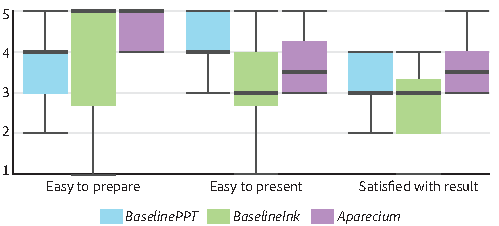
\includegraphics[width=1\columnwidth]{figures/study1likert}
        \caption{Summary of Likert responses from Study 1 on a scale from 1 (strongly disagree) to 5 (strongly agree).}
\label{fig:likert}
\end{figure}

%\definecolor{color1}{rgb}{0.92, 0.83, 0.78}
%\definecolor{color2}{rgb}{0.91, 0.66, 0.66}
%\definecolor{color3}{rgb}{0.68, 0.68, 0.96}
%\begin{figure}
%\centering
%\begin{tikzpicture}
%\begin{axis}[
%ybar,
%enlargelimits=0.15,
%enlarge y limits={upper=0},
%legend style={at={(0.5,-0.15)},
%  anchor=north,legend columns=-1},
%symbolic x coords={Easy Setup, Easy Delivery, Satisfaction},
%xtick=data,
%%    nodes near coords,
%%    nodes near coords align={vertical},
%scaled y ticks = false,
%ymin =0,
%ylabel={Score},
%]
%\addplot[style={fill=color1}, error bars/.cd, y dir=both, y explicit]
%coordinates {
%(Easy Setup, 3.6) += (0,1.0) -= (0,1.0)
%(Easy Delivery, 4.2) += (0,0.7) -= (0,0.7)
%(Satisfaction, 3.3)+= (0,0.8) -= (0,0.8)};
%\addplot[style={fill=color2}, error bars/.cd, y dir=both, y explicit] 
%coordinates {(Easy Setup, 3.9) += (0,0.2) -= (0,0.1)
%(Easy Delivery, 3.3) += (0,0.2) -= (0,0.1)
%(Satisfaction, 2.8)+= (0,0.2) -= (0,0.1)};
%\addplot[style={fill=color3}, error bars/.cd, y dir=both, y explicit] 
%coordinates {(Easy Setup, 4.6) += (0,0.2) -= (0,0.1)
%(Easy Delivery, 3.8) += (0,0.2) -= (0,0.1)
%(Satisfaction, 3.7)+= (0,0.2) -= (0,0.1)};
%\legend{BaselinePPT, BaselineInk, \interface (Ours)}
%\end{axis}
%\end{tikzpicture}
%\caption{Chart 1}
%\label{eval_chart1}
%\end{figure}
%
\textbf{\interface\ makes it easier to prepare slides.}\\
%\val{I feel like we should be more precise about the word preparation. Preparation can include studying the material, authoring the slide (plus setting up the slide--with animation effects etc), and rehearsing the slides. Here, I am trying to focus on the "set up part."}\\
Presenters found it easiest to set up the slides using our interface, followed by BaselineInk and then BaselinePPT (Figure~\ref{fig:likert}). With \interface, most presenters did not do any extra work (revealing or writing beforehand) to set up the slides, but used them as-is. In the few cases, where they pre-revealed parts of the foreground, they expressed that the required effort was minimal. 
%
In comparison, although our participants were familiar users of PowerPoint, they found the effort to set up animation effects tedious. To quote \textit{U6}, "\textit{It was cumbersome to add animations to each individual object and get the timing right... sometimes I decided I wanted to add an animation, but then had to figure out where to insert it in the existing animations sequence.}"
%
In terms of preparation effort, the BaselineInk condition was similar to our interface; most participants used the slide as-is, without writing additional content ahead of time. However, the reasons were different. In \interface, presenters had the ability to reveal the pre-authored foreground elements to the audience during the presentation. In the BaselineInk condition, presenters had to manually draw the foreground content, which they could either do ahead of time (thus losing the real-time effect) or during delivery. Either way, the effort was more \textit{"daunting"  (U12)} and  \textit{"time consuming" (U8)}, and the result was aesthetically less satisfactory (\textit{U1, U5, U8}).  
%%\val{Kruskall-Walis: chi-squared; 4.865, p = 0.0878}
%

\begin{figure}[t!]
    \centering
        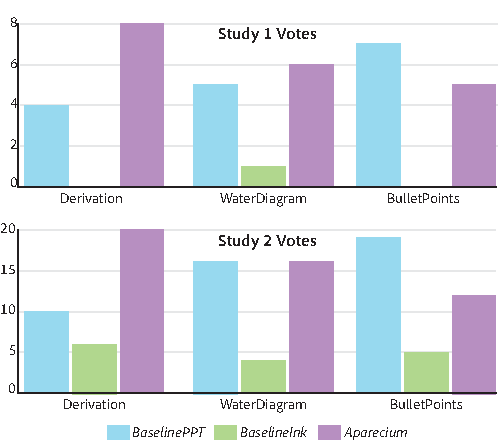
\includegraphics[width=1\columnwidth]{figures/studyVotes}
        \caption{Preferred tool/presentation for each content type.}
\label{fig:votes}
\end{figure}

\textbf{For presentation delivery, \interface\ involves comparable effort to BaslinePPT and less effort than BaselineInk.}\\
%{Kruskall-Walis chi squared: 4.044, p = 0.13}
%Presenters found it easiest to deliver the presentation using BaselinePPT, followed by our interface, and then BaselineInk. 
%
%The difference between BaselinePPT and our interface (Mann-Whitney U test: Z = 1.18, p = .24) was less significant than between that of BaselinePPT and BaselineInk (Z = -1.88, p = .06). \\
%
Regarding the ease of delivering presentations, BaselinePPT received slightly higher ratings than our interface. BaselineInk was rated the lowest by a larger margin. 
%
\wil{Although some reviewers do like statistical tests, I'm in the camp of just using descriptive statistics (e.g., means, quartiles, etc.) to present these types of results. Given how small our study is (and given that it is largely exploratory), I think that's more appropriate. If we all agree on this, we could say something to this effect earlier on to set expectations. } \val{Agreed. Where is a good place/what is a good way to say this?}
%
It is not surprising that BaselinePPT required the least effort. The only interaction presenters used was to press a single button to advance the slide animations. That said, when the animation involved more than a few steps, it was common for presenters to make mistakes. Three out of 12 participants forgot to advance the animation at the right time at least once, and only realized it at the next animation step. They had to either repeat the verbal explanation or quickly skip through the subsequent animations. In addition, two participants reported that they forgot to set up a desired animation step and only realized it during delivery. Several users suggested that having cues to help remember the animation would be beneficial $(U2, U7)$.

While presenters found inking in \interface\ straightforward, they noted that inking to reveal still required more effort than pushing a single button. Presenters seemed to prefer the path of minimum effort. For instance, with the exception of the math derivation content, they mostly used fast scribbling or strike-through gestures to reveal. As several presenters mentioned, this had the downside that the audience would initially see the scribbled ink strokes before the underlying pixels were revealed, which could potentially be distracting and aesthetically less pleasing. Some users suggested that they would prefer an even faster gesture such as clicking or circling to reveal large parts. On the other hand, they also expressed the idea that for the audience it could be better \textit{"to have the word appear after the inking instead of just after clicking like in powerpoint." (U1)} We discuss this tradeoff in more detail in the Limitations and Discussion section. %\val{I want to discuss the downsides of this path (e.g., less engaging for the audience, need setup (grouping of elements) but I don't want digress too much here.  What's a good phrase to signal the readers that we'll discuss this issue further later?}\wil{Maybe say that we discuss this tradeoff in more detail in Section X?}
%
In addition, users appreciated the automatic color selection for annotation and the modeless switching between revealing and inking. %\val{Should we mention here or in the Protocol, that space manipulation was not introduced the the participants for this study? Prefer in the protocol.}\wil{Agreed.}

As expected, BaselineInk required the most effort during delivery. Participants complained that drawing took away their attention from the content delivery. Since verbal explanations tend to be faster, there were periods of silence while the presenters were still drawing. In the Derivation presentation, three out of the four presenters who used BaselineInk ran out of space and had to use the margins or eraser. The one exception was a presenter who used the setup time to layout line numbers on the slide. In addition to these challenges, some users also complained about the specific difficulty of writing on a tablet. For example, the screen interface is not as smooth as paper \textit{(U1, U4, U6)} and operations such as switching to an eraser or a different color is tedious \textit{(U7, U9)}. 

\textbf{Presenters were most satisfied with the presentation quality of \interface\.}
Presenters were most satisfied with the presentation produced using \interface, followed by BaselinePPT and then BaselineInk. 
%
The difference in ratings between our interface and BaselinePPT was smaller than the difference between BaselinePPT and BaselineInk. \wil{Did I state this correctly? Again, I propose leaving out the statistical tests here.} \val{If we consider the "median", yes. If we consider the "mean", no.}
%
%The difference between our interface and BaselinePPT was less significant (Z = -0.95, p = .34) than that between ours and BaselineInk (Z = -1.88, p = 0.06). 
%
This trend held overall, as well as for each individual content type.

The feedback we gathered was consistent with our preliminary, formative interviews. Participants were accustomed to the BaselinePPT style, but in many cases they thought it could be improved with finer grained animation \textit{(U1, U3, U4, U8, U11)}. They liked the \textit{"handwritten in real time effect" (U4)}   in \interface, as it made the presentation \textit{"more interactive and seem to require engagement " (U9)}. The main complaints about BaselineInk presentations were that the drawings looked \textit{"messy" (U7)} and \textit{"not professional enough" (U6)}, and that the pace was too slow.

\textbf{Tool preference depends on presentation content.}
The tool preferences of both the presenters and audience depended on the content type. (Figure~\ref{fig:votes})
%
In Study 1, we asked presenters to choose which interface they would prefer to use for each content type.
%
For Derivation, presenters preferred  \interface\ (8/12) and then BaslineInk (4/12). For WaterDiagram, \interface\ (6/12) and BaslinePPT(5/12) were comparable choices. Similarly for BulletPoints, BaselinePPT (7/12) and \interface\ (5/12) were preferred.
%

In Study 2, we asked audiences which presentation was most engaging. For Derivation, the majority of audiences preferred \interface\ (20/36) followed by BaselinePPT (10/36) and then BaselineInk (6/36). For WaterDiagram, \interface\ (16/36) and BaselinePPT (16/36) were comparable. For BulletPoints audiences preferred BaselinePPT (19/36) and then \interface\ (12/36).
%
These findings confirm our intuition that fine-grained control of pace is most important for presenting sequential processes, especially for writing out text or equations (Derivation). In the case of the WaterDiagram, it was easy to achieve similar sized steps using BaselinePPT and \interface. The fact that the WaterDiagram slide consists mainly of images rather than text may have affected the users choice as well (see discussion about different ways to reveal). %\val{Here, or in a separate discussion, I want to bring up the observation that for Derivation, people used slow inking, but for WaterDiagram or BulletPoints, people used scribbling (even for revealing simple images such as clouds). There could be many reasons. e.g., presenter laziness; it's more difficult to draw the contour of an image; the image doesn't require much description, so it's not appropriate to take much time to draw. Should we talk about this in discussion section? It seems to lead to questions we can't answer here but rather interesting topics for future work. For example, if the presenters actually drew the contours of the image in the WaterDiagram, would audience preference be different? Is there a different "best revealing strategy" for different content type? Should we allow lasso for some types of contents? etc.} \wil{Maybe here we can say that the elements in WaterDiagram point out some potential limitations of our current reveal interactions (assuming we can refer to specific examples in the study where people seemed to have trouble revealing elements) and that we believe these could be addressed with extensions to our method, which we discuss more in future work.}
%
For simple lists and images (BulletPoint), BaselinePPT provided an appropriate pace and aesthetics.

\wil{Given that the overall message from the study results is pretty positive (generally easier for both preparation and delivery, and produces preferred results for some common content types), it would be nice to summarize this somewhere. Maybe as part of conclusions?} 


\section{Limitations and Discussion}
\val{In general, I had a hard time trying to group/order the contents in this section. The second part about interactivity seems less related to the other two. I almost feel like it's less relevant and that we should focus on 1 and 3 (No specific reason why it's ordered this way. }
\wil{I moved topic 2 to the end. I agree that it is less related than the other two but perhaps still nice to include.}
Here, we consider some limitations of our design, and discuss several observations and lessons learned about designing future presentation interfaces.

\textbf{Different Ways to Reveal.}  Several presenters in the first user study wanted an even quicker way than scribbling to reveal content. Indeed, scribbling over large areas to reveal images or long lines of text can be tedious, especially if the presenter is not concerned about simulating the real-time hand-drawn effect. 
%
In addition, some participants across both user studies complained that showing the scribbles before revealing the foreground elements is less aesthetically pleasing or even distracting. Conversely, other audience members commented that the scribbles served as helpful cues to draw attention to where information was about to appear. %The short transition time between when the scribbles appear and when the underlying elements are revealed can also give audiences time to turn their focus \val{I have not measured this time but I would say about 0.5sec. Should we mention this?}. \wil{I'm actually not clear about this point. Doesn't the transition time depend on how much scribbling is required? And what does it mean for audiences to turn their focus? Can we skip this last sentence?}
%
In general, supporting different types of revealing mechanisms (e.g., clicking or lasso selection) and allowing instantaneous reveal of certain elements could improve the presentation experience. However, such a design should not increase the preparation effort or limit flexibility during presentation.
%
For example, we considered allowing presenters to specify at setup time elements that can be revealed instantaneously upon clicking or tapping. However, this can make preparation tedious, akin to grouping elements and setting up animations in PowerPoint. Moreover, it does not allow presenters to change their mind during preparation about how to reveal elements. 

\textbf{Presenter Convenience vs. Presentation Quality.} The question of what revealing mechanisms to support points to a more fundamental tension with presenter interfaces. 
%
On the one hand, making the workflow more convenient for presenters is an important objective. However, it is at least as important to take into account the audience's point of view, since they are the intended consumers of the presentations themselves.
%
For example, providing a larger set of revealing gestures may tempt presenters to always opt for the minimum-effort gesture at the cost of presentation quality. In fact, in an earlier prototype of our system, we allowed revealing either by lasso selection or slow tracing, and observed that presenters almost always opted for the lasso tool even for the \textit{Derivation} type of content, which compromised presentation quality for the audience. Instead, we opted for a design that \textit{forces} the presenter to go at a slower pace.
%
More broadly, designing presentation tools that achieve the right balance between the needs of presenters and audience members remains an interesting direction for future work. In this vein, previous research that systematically compares the effect of different presentation styles (e.g.,~\cite{seth2010powerpoint, cross2013typerighting}) may provide valuable guidance for new interfaces that assist and \textit{nudge} presenters towards the most effective communication techniques.

\textbf{Creating Flexible Interactivity.} Our work focuses on presenting slides with static visuals, and \interface\ supports limited interaction with the displayed content (i.e., shifting elements to create empty space). In our formative interviews, several participants expressed the desire to present interactive content that can be controlled on-the-fly, for instance, to explain the steps of a computer algorithm or a physics diagram. 
%
While there are many existing approaches to creating interactive diagrams, designing authoring and presentation tools that are both convenient and flexible is a challenging problem that bears further exploration.

%\wil{I left out the references below. Not sure if we need them.\\
%\\
%Some previous approaches to creating interactive diagrams rely on domain specific knowledge \cite{laviola2007mathpad,alvarado2001preserving}. More general-purpose techniques create parameterized graphics and animations via programming~\cite{zongker2003creating} or visual authoring of simple state machines~\cite{kazi2014kitty}.
%}


\if 0
Presenter interfaces are inherently two-sided. On the one hand, it is easy to focus on the presenters since they are the direct users of the interface. However, it is equally, if not more, important to take into account the audience's point of view since they are the intended consumers of the output of the interface. As previously noted, presenters and audience may have conflicting interests. Presenters may prefer the easiest path, which may not be most informative path for the audience. Moreover, these preferences are context dependent. \val{point to our formative work?} Balancing the two sides can be tricky but also opens up opportunity. Works such as \cite{seth2010powerpoint, cross2013typerighting} that systematically compare the effect of different presentation styles can help. Also once we define effective presentation styles, designing interfaces that assist and \textit{nudge} the presenters to implement such styles is important. 

In general, finding the right balance between real-time drawing and instantaneous display that is both convenient for the presenter and appropriately paced for the audience is an interesting problem that bears further exploration.

Supporting different types of revealing mechanisms (e.g., clicking or lasso selection) and allowing instantaneous reveal of certain elements could improve the presentation experience. However, there are several trade-offs to consider.
%
One important consideration is to implement a design that does not increase the preparation effort or limit flexibility during presentation. For example, we considered allowing presenters to specify at setup time elements that can be revealed instantaneously upon clicking or tapping. However, this can make preparation tedious, akin to grouping elements and setting up animations in PowerPoint. Moreover, it does not allow presenters to change their mind during preparation about how to reveal elements. 
%
Another trade-off is between presenter convenience and the quality of the presentation. Providing a larger set of revealing gestures may tempt presenters to always opt for the minimum-effort gesture at the cost of presentation quality. In fact, in an earlier prototype of our system, we allowed revealing either by lasso selection or slow tracing, and observed that presenters almost always opted for the lasso tool even for the \textit{Derivation} type of content, which compromised presentation quality for the audience. Instead, we opted for a design that \textit{forces} the presenter to go at a slower pace.
%Anothere possibility is to implement a context aware revealing mechanism that analyzes the slide content and the presenters gesture to decide the best way to reveal (e.g., if the presenter draws a closed curve around an image, the entire image is revealed instantly). However, it is impossible to anticipate all the different use cases (e.g., the presenter may actually want to reveal a closed contour inside an image), and erroneous predictions can be harmful. \val{Maybe I should emphasize that "best way" is ambiguous, rather than the fact that the system might misinterpret the user's intent (which is how it reads now).}\\
\fi



\section{Conclusion}
This paper introduces \interface, a novel presentation interface that combines inking interactions with pre-authored slides to help presenters deliver flexible and engaging presentations.
%
Our modeless inking interactions allow presenters to reveal, annotate and create extra space during a presentation. We evaluated our interface from the perspective of presenters and the audience by comparing it against two baseline interfaces, representing conventional slide and inking tools. Presenters found our interface easy to use both during preparation and delivery. In particular, for text-heavy, process-driven content, both presenters and audience preferred presentations delivered using \interface. 
%
In light of these findings, we believe our inking interactions could be a valuable addition to existing slide-based presentation tools.

% BALANCE COLUMNS
\balance{}

% REFERENCES FORMAT
% References must be the same font size as other body text.
\bibliographystyle{SIGCHI-Reference-Format}
\bibliography{paper}

\end{document}

%%% Local Variables:
%%% mode: latex
%%% TeX-master: t
%%% End:
